\begin{frame}{目录}
    \tableofcontents
\end{frame}

\begin{section}{时序差分方法\alert{(Q-Learning)}}

\begin{frame}{从有模型到无模型}
    \begin{figure}
        \centering
        \includegraphics[width=0.6\textwidth]{assets/Figure_chapterMap.png}
    \end{figure}
\end{frame}

\begin{frame}{从有模型到无模型}
    回顾贝尔曼公式:
    \[
        v_\pi(s)=\sum_a\pi(a|s)\left[\sum_r p(r|s,a)r+\gamma\sum_{s'}p(s'|s,a)v_{\pi}(s')\right], \quad \forall s\in\mathcal{S}
    \]
    \begin{itemize}
        \item 有模型:$p(r|s,a)$和$p(s'|s,a)$已知;
        \item 无模型:$p(r|s,a)$和$p(s'|s,a)$未知。
    \end{itemize}
    对于给定的策略,贝尔曼公式可以在有模型的情况下计算出状态价值。

    无模型的情况下,如何估计状态价值——\alert{时序差分方法}。

\end{frame}

\begin{frame}{时序差分方法:TD}
    问题描述:
    \begin{itemize}
        \item 对于给定的策略$\pi$,估计状态价值$\{v_\pi(s)\}_{s\in \mathcal{S}}$
        \item 输入:一系列采样\alert{$(s_0, r_1, s_1,\cdots,s_t,r_{t+1},s_{t+1},\cdots)$}或$\{(s_t,r_{t+1},s_{t+1})\}_t$
    \end{itemize}
    重要标注:
    \[
        \begin{aligned}
            v(s)&\longrightarrow v_\pi(s) \\
            &\downdownarrows \\
            v(s_{\alert{t}})&\longrightarrow v_\pi(s_{\alert{t}}) \\
            &\downdownarrows \\
            v_{\alert{t}}(s_{\alert{t}}) &\longrightarrow v_\pi(s_{\alert{t}})
        \end{aligned}
    \]  
\end{frame}

\begin{frame}{时序差分方法:TD}
    \textbf{TD算法}:
    \setcounter{equation}{0}
    \begin{equation}
        v_{t+1}(s_t)=v_t(s_t)-\alpha[v_t(s_t)-(r_{t+1}+\gamma v_t(s_{t+1}))]
    \end{equation}
    \begin{equation}
        v_{t+1}(s)=v_t(s), \quad \forall s\neq s_t
    \end{equation}
    其中$t=0,1,2,..\cdots$

    此时,$v_t(s_t)$是$t$时刻对$v_\pi(s_t)$状态价值的估计;$\alpha$是学习率。
    \begin{itemize}
        \item 在$t$时刻,只有路过的状态$s_t$的价值$v_t(s_t)$会被更新,其他状态的价值与上一个时刻一致;
        \item 之后有时将省略(2)式。
    \end{itemize}
\end{frame}

\begin{frame}{时序差分方法:TD}
    TD算法的性质:
    \begin{itemize}
        \item TD算法只会估计对于给定策略的\alert{状态价值}。
        \begin{itemize}
            \item 它不会估计动作价值
            \item 它不会寻找最优策略
        \end{itemize}
        \item TD算法可以很容易地拓展到可以估计动作价值和寻找最优策略的形式。
        \item 后续的时序差分算法都将以TD为基础。
    \end{itemize}
    问题:TD算法在数学上解决了什么?

    答:TD算法可以在\alert{无模型}但是\alert{有样本}的时候求解以下贝尔曼方程:
    \[
        v_\pi(s)=\mathbbm{E}[R+\gamma v_\pi(S')|s], \quad \forall s\in\mathcal{S}
    \]

    (还记得有模型怎么求解吗?——矩阵向量形式,值迭代法)
\end{frame}

\begin{frame}{时序差分方法:Sarsa}
    \begin{itemize}
        \item TD算法只会估计对于给定策略的\alert{状态价值}。
        \item 接下来介绍的Sarsa算法可以直接估计动作价值。
        \item Sarsa算法也可以寻找最优策略。
    \end{itemize}
\end{frame}

\begin{frame}{时序差分方法:Sarsa}
    问题描述:
    \begin{itemize}
        \item 对于给定的策略$\pi$,估计所有的动作价值$\{q_\pi(s, a)\}_{s\in \mathcal{S}, a\in\mathcal{A}}$
        \item 输入:一系列采样\alert{$(s_0, a_0, r_1, s_1, a_1,\cdots,s_t, a_t, r_{t+1}, s_{t+1}, a_{t+1},\cdots)$}或$\{(s_t, a_t, r_{t+1}, s_{t+1}, a_{t+1})\}_t$
    \end{itemize}
    我们可以使用Sarsa算法估计动作价值:
    \[
        \begin{aligned}
            q_{t+1}(s,a)&=q_t(s,a)-\alpha[q_t(s,a)-(r_{t+1}+\gamma q_t(s_{t+1},a_{t+1}))] \\
            q_{t+1}(s,a)&=q_t(s,a), \quad \forall s\neq s_t, a\neq a_t
        \end{aligned}
    \]
    其中$t=0,1,2,..\cdots$
    \begin{itemize}
        \item $q_t(s_t,a_t)$是在$t$时刻对$q_\pi(s_t,a_t)$的估计。
        \item $\alpha$是学习率。
    \end{itemize}
\end{frame}

\begin{frame}{时序差分方法:Sarsa}
    \begin{itemize}
        \item \textbf{为什么这个算法被称作Sarsa?}因为这个算法的每一步都涉及到序列$(s_t, a_t, r_{t+1}, s_{t+1}, a_{t+1})$。Sarsa就是state-action-reward-state-action的简写形式。
        \item \textbf{Sarsa算法和TD算法之间是什么关系?}我们可以直接把TD算法中估计状态价值的$v_(s)$替换成估计动作价值的$q_(s,a)$。所以Sarsa算法是TD算法用于估计动作价值的一个拓展。
        \item \textbf{Sarsa算法在数学上解决了什么?}Sarsa算法可以在\alert{无模型}但是\alert{有样本}的时候求解以下贝尔曼方程:
        \[
            q_\pi(s,a)=\mathbbm{E}[R+\gamma q_\pi(S',A')|s,a], \quad \forall s\in\mathcal{S}, a\in\mathcal{A}
        \]
    \end{itemize}   
\end{frame}

\begin{frame}{时序差分方法:Sarsa}
    \begin{block}{Sarsa寻找最优策略}
        \begin{algorithmic}[1]
            \For{每一个轮次}
                \State 依据$\pi_0(s_0)$从初始状态$s_0$开始选择动作状态$a_0$
                \If{$s_t(t=0,1,2,\cdots)$不是目标状态}
                    \State 依据$(s_t,a_t)$收集样本$(r_{t+1},s_{t+1},a_{t+1})$:通过与环境交互获得$r_{t+1},s_{t+1}$,根据$\pi_t(s_{t+1})$获得$a_{t+1}$。
                    \State 更新$(s_t, a_t)$的动作价值:
                    \[
                        q_{t+1}(s_t,a_t)=q_t(s_t,a_t)-\alpha[q_t(s_t,a_t)-(r_{t+1}+\gamma q_t(s_{t+1},a_{t+1}))]
                    \]
                    \State \alert{更新策略$\pi_t(s_t)$}:
                    \[
                        \alert{\pi_{t+1}(s_t)=\arg\max_a q_{t+1}(s_t,a)}
                    \]
                \EndIf
            \EndFor
        \end{algorithmic}
    \end{block}
\end{frame}

\begin{frame}{$\epsilon$-greedy策略}
    假设网格世界中从起点出发到终点有以下两种轨迹:
    \begin{itemize}
        \item 轨迹A:很直接,容易发现,回报低(可能经过了一些禁止区域)
        \item 轨迹B:需要绕来绕去,很难发现,但是回报高
    \end{itemize}
    但是根据上一页的算法,智能体就很容易就会陷入轨迹A,永远探索不到轨迹B。
    \begin{block}{$\epsilon$-greedy策略}
        \[
            \pi(a|s)=\begin{cases}
                1-\frac{\epsilon}{|\mathcal{A}|}(|\mathcal{A}|-1),\quad a=\arg\max_{a}q(s,a) \\
                \frac{\epsilon}{|\mathcal{A}|},\quad a \neq \arg\max_{a}q(s,a)
            \end{cases}
        \]
    \end{block}
    \begin{itemize}
        \item 例:在网格世界中,$\epsilon=0.1$,则有$92\%$的概率选择最优动作,$2\%$的概率随机选择其他动作中的任意一个。
    \end{itemize}
\end{frame}

\begin{frame}{时序差分方法:Sarsa}
    Sarsa算法的特点:
    \begin{itemize}
        \item 状态$s_t$的策略在$q(s_t,a_t)$更新之后立刻就更新了。所以它是一个增量更新的算法,不需要收集整条轨迹才更新一次策略。
        \item Sarsa算法需要使用$\epsilon$-greedy策略来平衡探索和利用。
    \end{itemize}
    Sarsa算法的核心:
    \begin{itemize}
        \item Sarsa算法的核心很简单:求解贝尔曼方程。
        \[
            q_\pi(s,a)=\mathbbm{E}[R+\gamma q_\pi(S',A')|s,a], \quad \forall s\in\mathcal{S}, a\in\mathcal{A}
        \]
        \item Sarsa算法有可能会看起来复杂,是因为实际写成代码的时候需要考虑算法效率和更新策略。
    \end{itemize}
\end{frame}

\begin{frame}{时序差分方法:Sarsa}
    例子:
    \begin{itemize}
        \item 问题:找到从一个\alert{特定的起点}走到终点的好路径。
        \begin{itemize}
            \item 这个问题和之前问题的不同之处在于,我们并不需要找出\alert{所有状态的最优策略}。
            \item 每一条轨迹的起点都是左上角,终点都是target
        \end{itemize}
        \item $r_{\text{boundary}}=r_{\text{forbidden}}=-10, r_{\text{target}}=0, r_\text{other}=-1, \gamma=0.9, \alpha=0.1, \epsilon=0.1$
    \end{itemize}
\end{frame}

\begin{frame}{时序差分方法:Sarsa}
    结果:
    \begin{itemize}
        \item 左图是Sarsa找到的最优策略
        \begin{itemize}
            \item \alert{注意并不是所有状态都是最优策略。}
        \end{itemize}
        \item 右图是每一轮迭代的回报和轨迹长度。
    \end{itemize}
    \begin{center}
        \begin{minipage}{0.35\textwidth}
            \centering
            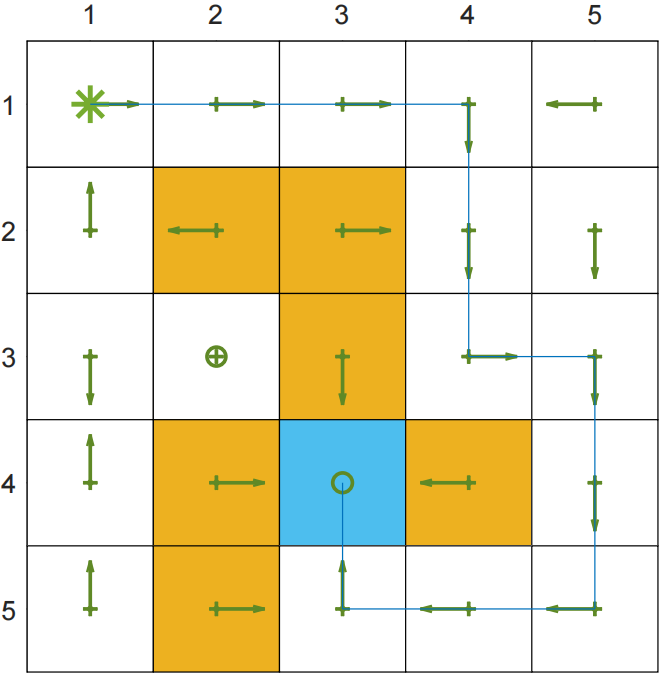
\includegraphics[width=\linewidth]{assets/SarsaPolicy.jpg}
        \end{minipage}
        \hspace{1cm}
        \begin{minipage}{0.35\textwidth}
            \centering
            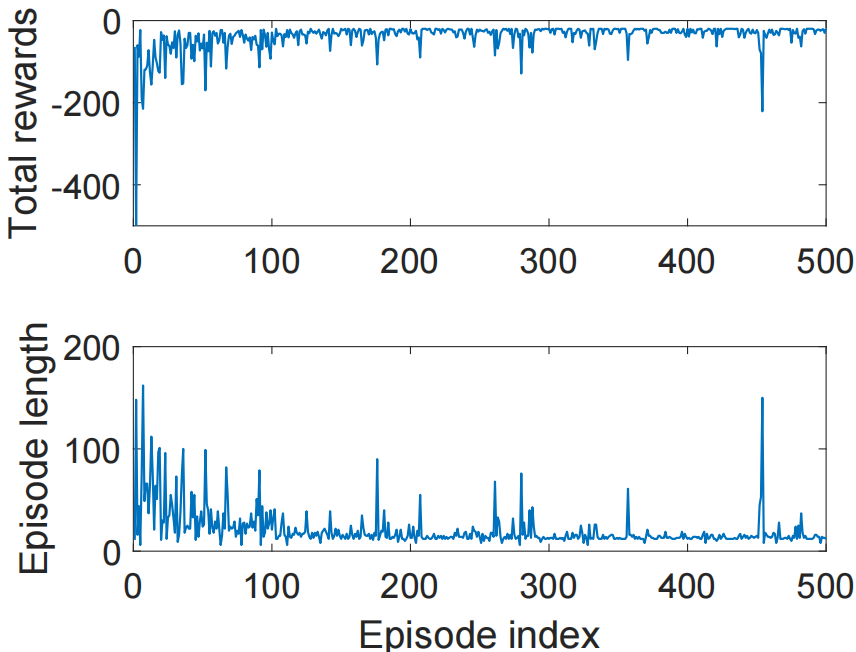
\includegraphics[width=\linewidth]{assets/SarsaReward.jpg}
        \end{minipage}
    \end{center}
\end{frame}

\begin{frame}{时序差分方法:n步Sarsa}
    动作价值的定义:
    \[
        q_\pi(s,a)=\mathbbm{E}(G_t|S_t=s, A_t=a)
    \]
    折扣回报$G_t$可以被写为:
    \[
        \begin{aligned}
            \text{Sarsa}\longleftarrow G_t^{(1)}&=R_{t+1}+\gamma q_\pi(S_{t+1}, A_{t+1}), \\
            G_t^{(2)}&=R_{t+1}+\gamma R_{t+2}+ \gamma^2 q_\pi(S_{t+2}, A_{t+2}), \\
            &\vdots \\
            \alert{\text{n步Sarsa}}\longleftarrow G_t^{(n)}&=R_{t+1}+\gamma R_{t+2}+ \gamma^2 R_{t+3} + \cdots+\gamma^n q_\pi(S_{t+n}, A_{t+n}), \\
            &\vdots \\
            \text{Monte Carlo}\longleftarrow G_t^{(\infty)}&=R_{t+1}+\gamma R_{t+2}+\gamma^2 R_{t+3}+\cdots
        \end{aligned}
    \]
\end{frame}

\begin{frame}{时序差分方法:n步Sarsa}
    Sarsa要解的方程:
    \[
        q_\pi(s,a)=\mathbbm{E}[G_t^{(1)}|s, a]=\mathbbm{E}[R_{t+1}+\gamma q_\pi(S_{t+1}, A_{t+1})|s, a]
    \]
    Monte Carlo要解的方程:
    \[
        q_\pi(s,a)=\mathbbm{E}[G_t^{(\infty)}|s, a]=\mathbbm{E}[R_{t+1}+\gamma R_{t+2}+\gamma^2 R_{t+3}+\cdots|s, a]
    \]
    \alert{n步Sarsa要解的方程:}
    \[
        q_\pi(s,a)=\mathbbm{E}[G_t^{(n)}|s, a]=\mathbbm{E}[R_{t+1}+\gamma R_{t+2}+\cdots+\gamma^n q_\pi(S_{t+n}, A_{t+n})|s, a]
    \]
    \begin{itemize}
        \item 在$n=1$时,n步Sarsa就是Sarsa
        \item 在$n\rightarrow\infty$时,n步Sarsa就是Monte Carlo
    \end{itemize}
\end{frame}

\begin{frame}{时序差分方法:n步Sarsa}
    \begin{itemize}
        \item 输入:n步Sarsa需要$(s_t,a_t,r_{t+1},s_{t+1},a_{t+1},\cdots,r_{t+n},s_{t+n},a_{t+n})$
        \item 在$t$时刻,$(r_{t+n},s_{t+n},a_{t+n})$还没有发生,所以我们无法在t时刻就立刻更新$q(s_t, a_t)$,需要等到$t+n$时刻才能更新$q(s_t,a_t)$:
        \[
            \begin{aligned}
                q_{t+n}(s_t,a_t)=&q_{t+n-1}(s_t, a_t)\\
                &-\alpha[q_{t+n-1}(s_t,a_t)-[r_{t+1}+\gamma r_{t+2}+\cdots+\gamma^nq_{t+n-1}(s_{t+n}, a_{t+n})]]
            \end{aligned}
        \]
        \item n步Sarsa是Sarsa和Monte Carlo的折衷算法:
        \begin{itemize}
            \item Sarsa算法收敛过程波动很小,收敛结果偏差很大;
            \item Monte Carlo算法收敛过程波动很大,收敛结果偏差很小;
            \item n步Sarsa算法收敛过程的波动和收敛结果的偏差比较适中。
        \end{itemize}
    \end{itemize}
\end{frame}

\begin{frame}{时序差分方法:\alert{Q-Learning}}
    \begin{itemize}
        \item 接下来我们介绍\alert{Q-Learning},它直到今天也是最常用的强化学习算法。
        \item Sarsa可以对给定的策略$\pi$估计其相应的动作价值。它必须需要伴随着一个逐步迭代的路径来更新它的估计和策略。
        \item \alert{Q-Learning}可以直接估计最优的动作价值和最优策略。
    \end{itemize}
\end{frame}

\begin{frame}{时序差分方法:Q-Learning}
    Sarsa算法:
    \[
        q_{t+1}(s,a)=q_t(s,a)-\alpha[q_t(s,a)-(r_{t+1}+\gamma \alert{q_t(s_{t+1},a_{t+1})})]
    \]
    \textbf{Q-Learning算法:}
    \[
        q_{t+1}(s,a)=q_t(s,a)-\alpha[q_t(s,a)-(r_{t+1}+\gamma \alert{\underset{a\in\mathcal{A}}{\max}q_t(s_{t+1},a)})]
    \]
    Q-Learning和Sarsa算法非常相似,只是它们的收敛目标不一样。
    \begin{itemize}
        \item Sarsa算法中的收敛目标是$r_{t+1}+\gamma \alert{q_t(s_{t+1},a_{t+1})}$。
        % 其中$q_{t+1}$是根据给定策略$\pi_t(s_{t+1})$生成的。
        \item Q-Learning算法中的收敛目标是$r_{t+1}+\gamma \alert{\underset{a\in\mathcal{A}}{\max}q_t(s_{t+1},a)}$。
        % 其中$a$是根据最优策略$\pi^*_t(s_{t+1})$生成的。
    \end{itemize}
\end{frame}

\begin{frame}{时序差分方法:Q-Learning}
    \textbf{Q-Learning要解的方程:}
    \[
        q(s,a)=\mathbbm{E}[R_{t+1}+\gamma\underset{a}{\max}q(s_{t+1}, a)| S_t=s, A_t=a], \quad \forall s,a
    \]
    这是一个贝尔曼\alert{最优}方程用动作价值表达的形式。

    所以Q-Learning可以直接估计出\alert{最优(策略对应)的动作价值},而不是某一特定策略的动作价值。
\end{frame}

\begin{frame}{时序差分方法:Q-Learning}
    \vspace{-0.2cm}
    \begin{block}{Q-Learning寻找最优策略}
        \begin{algorithmic}[1]
            \setlength{\baselineskip}{0.5\baselineskip}
            \For{对于收集到的每一个经验样本$(s_t, a_t, r_{t+1}, s_{t+1})$}
                \State 更新$(s_t, a_t)$的动作价值:

                $
                    q_{t+1}(s_t,a_t)=q_t(s_t,a_t)-\alpha[q_t(s_t,a_t)-(r_{t+1}+\gamma \underset{a}{\max}q_t(s_{t+1},a))]
                $
                \State 更新策略$\pi_t(s_t)$(greedy):

                $
                    \pi_{t+1}(s_t)=\arg\max_a q_{t+1}(s_t,a)
                $
                \State 更新策略$\pi_t(s_t)$($\epsilon$-greedy):
                
                $
                    \pi_{t+1}(a|s_{t})=\begin{cases}
                        1-\frac{\epsilon}{|\mathcal{A}|}(|\mathcal{A}|-1),\quad a=\arg\max_{a}q_{t+1}(s_t,a) \\
                        \frac{\epsilon}{|\mathcal{A}|},\quad a \neq \arg\max_{a}q_{t+1}(s_t,a)
                    \end{cases}
                $
            \EndFor
        \end{algorithmic}
    \end{block}
\end{frame}

\begin{frame}{时序差分方法:Q-Learning}
    什么时候选择greedy?什么时候选择$\epsilon$-greedy?
    
    输入的经验样本集合$\{(s_t, a_t, r_{t+1}, s_{t+1})\}_n$来源于哪里?
    \begin{itemize}
        \item 依据$\pi_t$生成的。在$t$时刻想要更新状态$s_t$中某一个动作的动作价值,就把$s_t$输入到当前的$\pi_t$中,得到$a_t$,然后通过与环境交互得到$(r_{t+1},s_{t+1})$;\alert{——{$\epsilon$}-greedy}
        \item 依据一个别的任意策略$\pi_b$生成的。在$t$时刻想要更新状态$s_t$中某一个动作的动作价值,就把$s_t$输入到一个固定的策略$\pi_b$中,得到$a_t$,然后通过与环境交互得到$(r_{t+1},s_{t+1})$;\alert{——greedy}
        \item 随机生成的。在$t$时刻想要更新状态$(s_t,a_t)$的动作价值,就直接通过与环境交互得到$(r_{t+1},s_{t+1})$;\alert{——greedy}
    \end{itemize}
    Q-Learning可以从别的策略产生的经验中学习,这种特性叫做off-policy。之前我们所学的TD和Sarsa都是on-policy的算法。
\end{frame}

\begin{frame}{时序差分方法:Q-Learning}
    例子:
    \begin{itemize}
        \item 问题:找到从\alert{所有的起点}走到终点的最优路径。
        \item $r_{\text{boundary}}=r_{\text{forbidden}}=-1, r_{\text{target}}=1, r_\text{other}=0, \gamma=0.9, \alpha=0.1$
    \end{itemize}
    真实值:
    \begin{center}
        \begin{minipage}{0.3\textwidth}
            \centering
            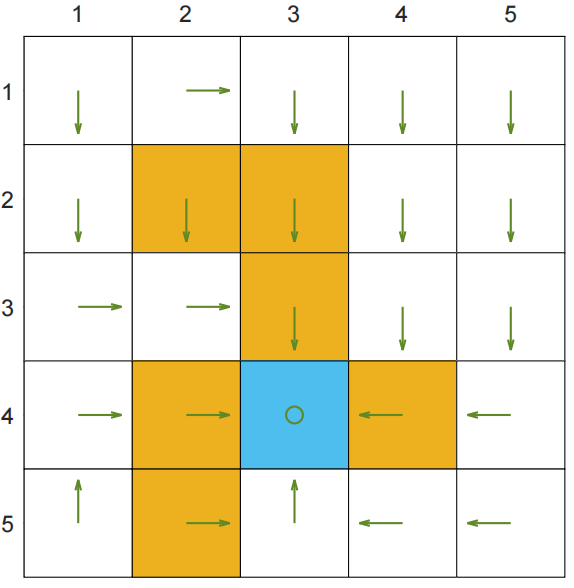
\includegraphics[width=\linewidth]{assets/OptimalPolicy.jpg}
            \captionof{figure}{最优策略}
        \end{minipage}
        \hspace{1cm}
        \begin{minipage}{0.3\textwidth}
            \centering
            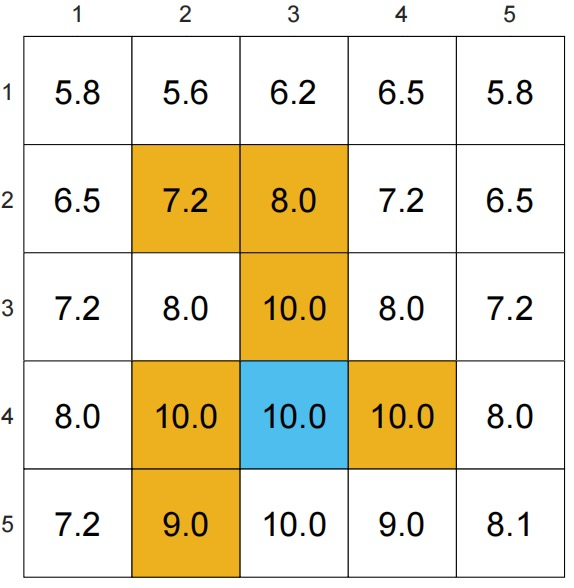
\includegraphics[width=\linewidth]{assets/OptimalStateValue.jpg}
            \captionof{figure}{最优状态价值}
        \end{minipage}
    \end{center}
\end{frame}

\begin{frame}{时序差分方法:Q-Learning}
    生成策略、生成的经验样本通过off-policy方式的Q-Learning学习到的策略($10^5$步):
    \begin{center}
        \begin{minipage}{0.2\textwidth}
            \centering
            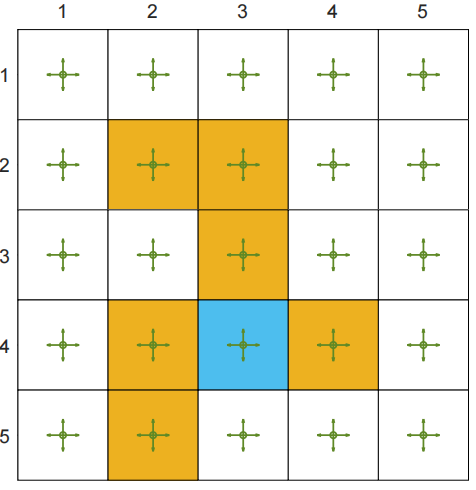
\includegraphics[width=\linewidth]{assets/e1policy.jpg}
            \captionof{figure}{生成策略}
        \end{minipage}
        \hspace{1cm}
        \begin{minipage}{0.2\textwidth}
            \centering
            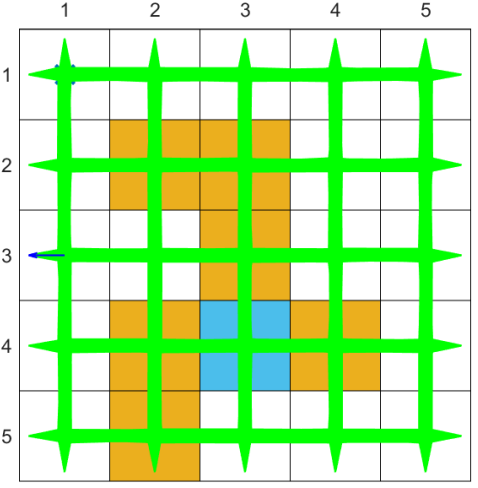
\includegraphics[width=\linewidth]{assets/e1episode.jpg}
            \captionof{figure}{生成策略的轨迹}
        \end{minipage}
        \hspace{1cm}
        \begin{minipage}{0.2\textwidth}
            \centering
            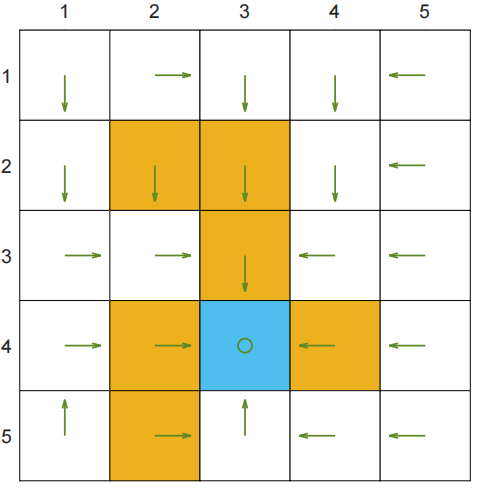
\includegraphics[width=\linewidth]{assets/e1qpolicy.jpg}
            \captionof{figure}{学习策略}
        \end{minipage}
        \hspace{1cm}
        \begin{minipage}{0.2\textwidth}
            \centering
            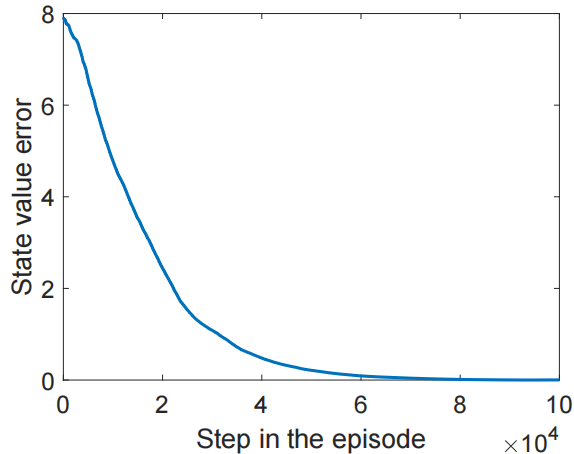
\includegraphics[width=\linewidth]{assets/e1statevalueerror.jpg}
            \captionof{figure}{状态价值误差}
        \end{minipage}
    \end{center}
\end{frame}

\begin{frame}{时序差分方法:Q-Learning}
    探索的重要性:$10^5$步

    如果生成策略探索得不充分,得到的经验样本就会很差。
    \begin{center}
        \begin{minipage}{0.2\textwidth}
            \centering
            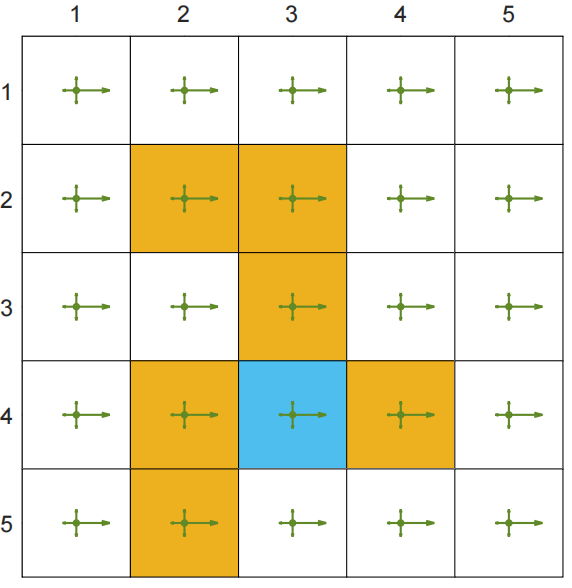
\includegraphics[width=\linewidth]{assets/e0.5policy.jpg}
            \captionof{figure}{生成策略$\epsilon=0.5$}
        \end{minipage}
        \hspace{1cm}
        \begin{minipage}{0.2\textwidth}
            \centering
            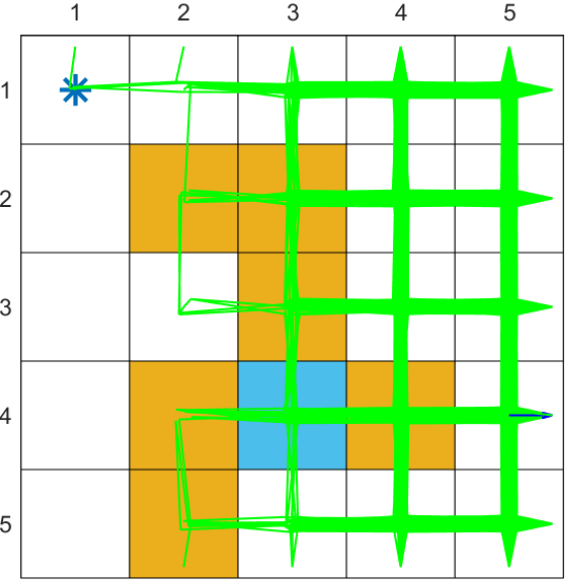
\includegraphics[width=\linewidth]{assets/e0.5episode.jpg}
            \captionof{figure}{生成策略的轨迹}
        \end{minipage}
        \hspace{1cm}
        \begin{minipage}{0.2\textwidth}
            \centering
            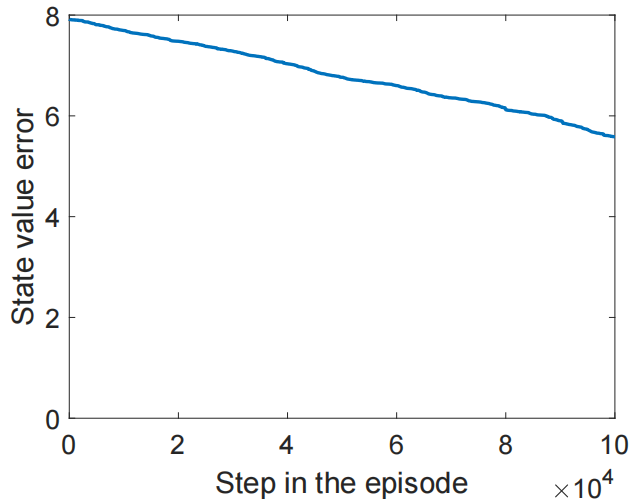
\includegraphics[width=\linewidth]{assets/e0.5statevalueerror.jpg}
            \captionof{figure}{状态价值误差}
        \end{minipage}
        \hspace{1cm}
    \end{center}
\end{frame}

\begin{frame}{时序差分方法:Q-Learning}
    \begin{center}
        \begin{minipage}{0.2\textwidth}
            \centering
            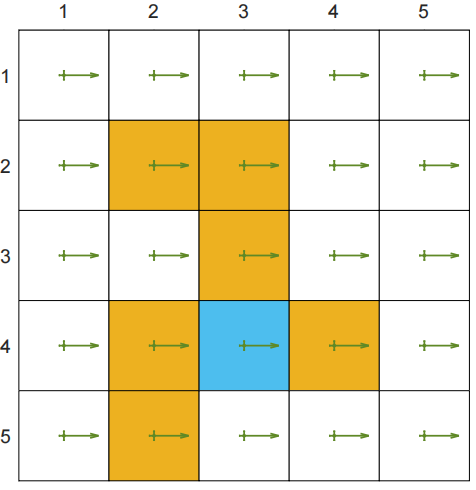
\includegraphics[width=\linewidth]{assets/e0.1policy.jpg}
            \captionof{figure}{生成策略$\epsilon=0.1$}
        \end{minipage}
        \hspace{1cm}
        \begin{minipage}{0.2\textwidth}
            \centering
            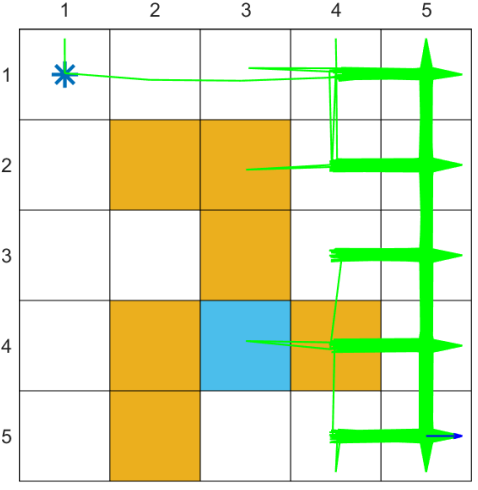
\includegraphics[width=\linewidth]{assets/e0.1episode.jpg}
            \captionof{figure}{生成策略的轨迹}
        \end{minipage}
        \hspace{1cm}
        \begin{minipage}{0.2\textwidth}
            \centering
            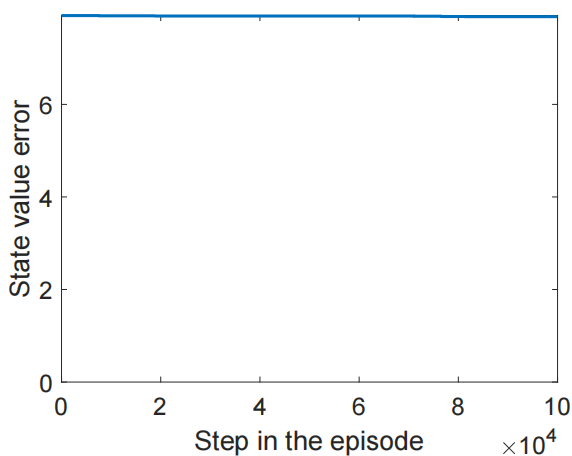
\includegraphics[width=\linewidth]{assets/e0.1statevalueerror.jpg}
            \captionof{figure}{状态价值误差}
        \end{minipage}
    \end{center}

    \begin{center}
        \begin{minipage}{0.2\textwidth}
            \centering
            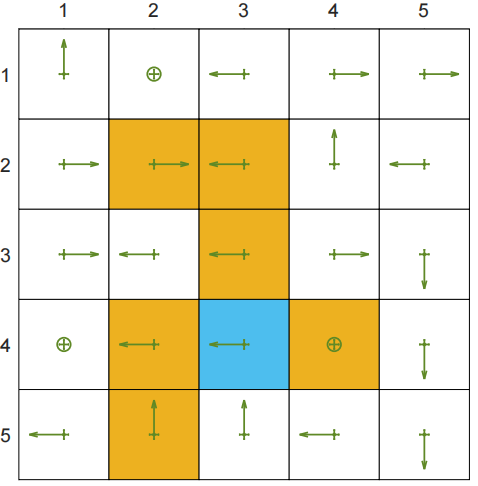
\includegraphics[width=\linewidth]{assets/e0.1policy2.jpg}
            \captionof{figure}{生成策略$\epsilon=0.1$}
        \end{minipage}
        \hspace{1cm}
        \begin{minipage}{0.2\textwidth}
            \centering
            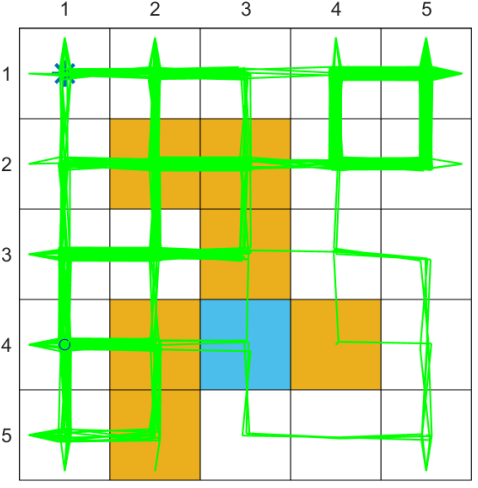
\includegraphics[width=\linewidth]{assets/e0.1episode2.jpg}
            \captionof{figure}{生成策略的轨迹}
        \end{minipage}
        \hspace{1cm}
        \begin{minipage}{0.2\textwidth}
            \centering
            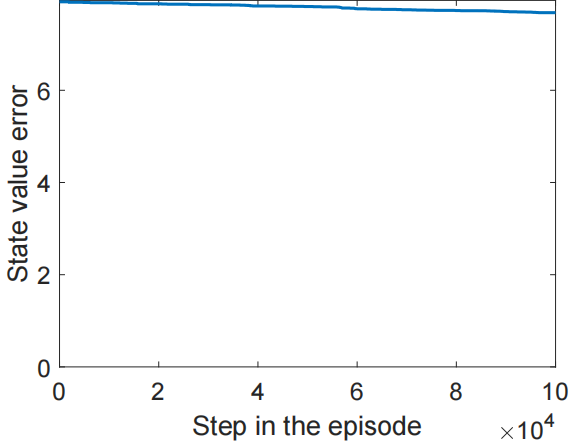
\includegraphics[width=\linewidth]{assets/e0.1statevalueerror2.jpg}
            \captionof{figure}{状态价值误差}
        \end{minipage}
    \end{center}
\end{frame}

\begin{frame}{小结}
    本节所有算法都可以归纳为以下形式:
    \[
        \alert{q_{t+1}(s,a)=q_t(s,a)-\alpha[q_t(s,a)-q_{\text{target}}]}
    \]
    其中$q_{\text{target}}$是时序差分算法求解的目标。
    \begin{table}[]
        \begin{tabular}{@{}cc@{}}
        \toprule
        算法    & $q_{\text{target}}$\\ \midrule
        Sarsa &  $r_{t+1}+\gamma q_t(s_{t+1}, a_{t+1})$\\
        n步Sarsa & $r_{t+1}+\gamma r_{t+2} + \cdots + \gamma^nq_t(s_{t+n},a_{t+n})$ \\
        Monte Carlo &  $r_{t+1}+\gamma r_{t+2} + \cdots$\\
        Q-Learning &  $r_{t+1}+\gamma \underset{a}{\max}q_t(s_{t+1}, a)$\\
        \bottomrule
        \end{tabular}
    \end{table}
\end{frame}

\begin{frame}{小结}
    所有时序差分算法都是解某种形式的贝尔曼公式的随机近似算法。
    \begin{table}[]
        \begin{tabular}{@{}cc@{}}
        \toprule
        算法    & 求解的方程\\ \midrule
        Sarsa &  BE:$q_\pi(s,a)=\mathbbm{E}[R_{t+1}+\gamma q_\pi(S_{t+1}, A_{t+1})|S_t=s,A_t=a]$\\
        n步Sarsa & BE:$q_\pi(s,a)=\mathbbm{E}[R_{t+1}+\gamma R_{t+1}+\cdots+\gamma^n q_\pi(S_{t+n}, A_{t+n})|S_t=s,A_t=a]$ \\
        Monte Carlo &  BE:$q_\pi(s,a)=\mathbbm{E}[R_{t+1}+\gamma R_{t+2}+\cdots|S_t=s,A_t=a]$\\
        Q-Learning & \alert{BOE:$q_\pi(s,a)=\mathbbm{E}[R_{t+1}+\gamma \underset{a}{\max}q_\pi(S_{t+1}, a)|S_t=s,A_t=a]$}\\
        \bottomrule
        \end{tabular}
    \end{table}
\end{frame}

\end{section}